\documentclass[12pt]{article}
\usepackage[utf8]{inputenc}
\usepackage[brazilian]{babel}
\usepackage{hyperref}
\usepackage{lipsum}
\usepackage{geometry}
\usepackage[skip=5pt plus1pt, indent=20pt]{parskip}
\usepackage{indentfirst}
\usepackage{graphicx}
\usepackage[center]{caption}
\usepackage[font=small]{caption}
\usepackage{subcaption}
\usepackage{placeins}
\usepackage{setspace}
\usepackage{amsthm,amssymb,amsmath}
\usepackage{algorithm}
\usepackage{algpseudocode}

\renewcommand*\familydefault{\sfdefault} 

\graphicspath{{./midia/}}

\geometry{margin=2cm}

\title{\textbf{Trabalho Prático 1 - Aritmofobia}}
\author{\textbf{Lucas Almeida Santos de Souza - 2021092563\textsuperscript{1}}}
\date{\parbox{\linewidth}{\centering%
	\textsuperscript{1}Universidade Federal de Minas Gerais (UFMG)\endgraf
	Belo Horizonte - MG - Brasil\endgraf\bigskip
	\href{mailto:luscaxalmeidass@ufmg.br}{luscaxalmeidass@ufmg.br}}}

\begin{document}

\maketitle

%%%%%%%%%%%%%%%%%%%%%%%%%%%%%%%%%%%%%%%%%%%%%%%%%%%%%%%%%%%%%%%%%%%%%%%%%%%%%%

\section{Introdução}

	\par O trabalho consiste na resolução de um problema envolvendo grafos em que é preciso encontrar um caminho entre dois vértices de um grafo. O caminho deve 1-ter peso par, 2-passar apenas por arestas de peso par e 3-passar por um número par de arestas.

	\par A entrada do programa desenvolvido consiste de um arquivo em que a primeira linha contém o número de vértices e o número de arestas do grafo separados por espaço e as linhas seguintes indicam as arestas do grafo, com o vértice de origem, o vértice de destino e o peso da aresta. A saída do programa é um arquivo contendo apenas um número que indica o peso do caminho encontrado, ou -1 caso não exista um caminho que satisfaça as condições.

\section{Modelagem}

	\par Para a implementação do grafo, foi utilizada a representação de lista de adjacências utilizando um vetor de tamanho n representando os vértices do grafo, com um vetor em cada posição representando as adjacências de cada vértice. Esse vetor de adjacências armazena um par \texttt{(w, p)}, onde \texttt{w} é o vizinho do vértice e \texttt{p} é o peso da aresta que liga o vértice a esse vizinho. Podemos ver um exemplo dessa representação abaixo:

	\begin{figure}[H]
		\centering
		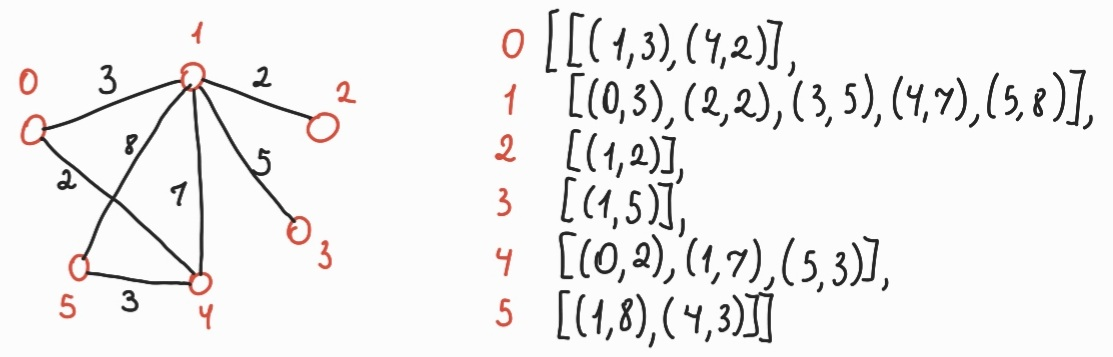
\includegraphics[width=0.8\textwidth]{exemplo_grafo.jpg}
		\caption{Representação da estrutura do grafo em lista de adjacências}
		\label{exemplo_grafo}
	\end{figure}

	\par Na Figura \ref{exemplo_grafo} os vizinhos de cada nó estão ordenados, mas isso não é necessário para o funcionamento do programa. Um detalhe adicional a ser considerado é que o grafo recebido é iniciado em 1, porém, para facilitar a implementação, cada vértice é subtraído por 1 durante a leitura do arquivo, fazendo com que o grafo seja iniciado em 0.

	\subsection*{Algoritmo}
		
		\par Para resolver o problema, foi utilizada uma variação do algoritmo de Dijkstra, além de uma restrição no momento de leitura do grafo. Ao ler uma aresta ímpar do arquivo de entrada, o programa main ignora e não a adiciona no grafo. Assim, a segunda condição já é satisfeita, pois o algoritmo nunca passará por arestas de peso ímpar.

		\par Para evitar confusões, a expressão "caminho par" será utilizada para indicar um caminho com número par de arestas, pois como todas as arestas válidas são pares, todos os caminhos possíveis já terão peso par.
		
		\par A variação do algoritmo de Dijkstra conta com uma estrutura chamada caminhos, que substitui o vetor original de distâncias. Ele consiste de um vetor de \texttt{pair} onde, para cada posição (vértice) o primeiro elemento do \texttt{pair} corresponde ao peso do caminho par mais curto e o segundo elemento corresponde ao peso do caminho ímpar mais curto. O vetor de visitados original do Dijkstra também sofreu uma alteração, agora contabilizando se o vértice foi visitado por um caminho par e/ou ímpar.

		\par Antes de percorrer os vértices, o programa inicializa todos os caminhos como $\infty$ e todos os visitados como false, pois assim qualquer caminho até um vértice será menor que o armazenado. O algoritmo inicia no primeiro vértice, que já contém um caminho par até ele mesmo de peso 0 e 0 arestas, e adiciona em todos os seus vizinhos (que têm $\infty$ como menor distância ímpar) a distância ímpar até ele como menor distância par até eles. Isso é feito pois, como o caminho até o primeiro vértice é par, o caminho até seus vizinhos é ímpar.
		
		\par Essa é a questão mais importante: para cada vértice, um caminho \textbf{par} até ele indica um caminho \textbf{ímpar} até seus vizinhos, passando por ele. Por isso, mesmo que estejamos buscando o menor caminho par até o destino, precisamos armazenar o menor caminho ímpar para cada vértice, pois ele pode fazer parte do menor caminho par até o destino. Por isso, o algoritmo armazena os dois caminhos para cada vértice.

		\subsubsection*{Complexidade}
		\par Essa variação do aloritmo de Dijkstra percorre a lista de prioridade e, para cada vértice, percorre seus vizinhos em busca do menor caminho. Mesmo podendo percorrer os vértices mais de uma vez, esse valor não cresce proporcionalmente à quantidade de vértices e arestas, então podemos assumir a complexidade assintótica de $O(n+m)$, assim como o algoritmo de Dijkstra, adicionada às ordenações da lista de prioridade que ocorrem em $O(logn)$. Assim, temos que a complexidade geral do algoritmo é $O(m+nlogn)$
	
	\subsection*{Pseudocódigo}
		
		\par O pseudocódigo do algoritmo é apresentado abaixo:
		
		\newpage
		\hrule
		\vspace{3pt}
		\hrule
		\noindent\textbf{Jodds( ):}
		
		\noindent\begin{tabular}{l}
			origem := 0, final := $n-1$ \\ \\
			caminhos := [($\infty$, $\infty$)] \footnotesize \textit{// Vetor com os pares de caminhos (par, ímpar) inicializados em ($\infty$, $\infty$)} \\
			caminhos[origem].par := 0 \footnotesize \textit{// O menor caminho par até a origem tem 0 arestas e peso 0} \\ \\
			visitados := [(false, false)] \footnotesize \textit{// Vetor com os pares de visitados (par, ímpar) inicializados em (false, false)} \\
			visitados[origem].par := true \footnotesize \textit{// A origem é visitada no caminho par} \\ \\
			fila.push(caminhos[origem].menor, origem) \footnotesize \textit{// Adiciona a origem na fila de prioridade } \\
			\textbf{enquanto} fila não está vazia \textbf{faça} \\
			\indent v := fila.top( ) \\
			\indent fila.pop( ) \\ \\
			\indent \textbf{se} visitado[v] == (true, true) \textbf{faça} \\
			\indent \indent \textbf{se} v for final \textbf{faça} \\
			\indent \indent \indent break \footnotesize \textit{// Se o vértice é final e já foi visitado nos dois caminhos, encerra o loop} \\
			\indent \indent \textbf{fim se} \\
			\indent \indent continue \footnotesize \textit{// Se o vértice já foi visitado nos dois caminhos, não analisa seus vizinhos} \\
			\indent \textbf{fim se} \\ \\
			\indent \textbf{para cada} vizinho w \textbf{de} v \textbf{faça} \\
			\indent \indent \textbf{se} (caminhos[v].par + o peso da aresta vw) $<$ caminhos[w].impar \textbf{faça} \\
			\indent \indent \indent caminhos[w].impar := (caminhos[v].par + o peso da aresta vw) \\
			\indent \indent \indent visitados[w].ímpar := true \\
			\indent \indent \indent visitados[w].par := false \\
			\indent \indent \textbf{fim se} \\
			\indent \indent \textbf{se} (caminhos[v].impar + o peso da aresta vw) $<$ caminhos[w].par \textbf{faça} \\
			\indent \indent \indent caminhos[w].par := (caminhos[v].impar + o peso da aresta vw) \\
			\indent \indent \indent visitados[w].par := true \\
			\indent \indent \indent visitados[w].ímpar := false \\
			\indent \indent \textbf{fim se} \\
			\indent \indent \textbf{se} algum caminho até w foi atualizado \textbf{faça} \\
			\indent \indent \indent fila.push(caminhos[w].menor, w) \\
			\indent \indent \textbf{fim se} \\
			\indent \textbf{fim para cada} \\ \\
			\textbf{fim enquanto} \\
			\textbf{se} caminhos[final].par != $\infty$ \textbf{faça} \\
			\indent \textbf{retorne} caminhos[final].dp \\
			\textbf{senão} \\
			\indent \textbf{retorne} -1 \\
			\textbf{fim se} \\
		\end{tabular}
		\hrule
		\vspace{3pt}
		\hrule
\end{document}